\section{问题三的模型建立与求解}

问题三延续问题二的附录 3 变物性模型和固定半径条件，定义连续重构场 $C_h(r,t)$ 的最大值函数
\[
 g(t)=\max_{0\le r\le R_0}C_h(r,t)-0.15.
\]
事件时刻是 $g(t)$ 从正值到负值的首次交点。计算先以 600 s 输出扫描括区间，再在事件区间内用 Brent 求根；空间上采用中心、表面和内部加密采样，避免把有限个输出点的最小值误当作全域判定。

正式结果为
\[
 t_*=57.47406473\,\mathrm h=206906.633\,\mathrm s.
\]
事件处最大含水率为 $0.1500000000\,\mathrm{kg/kg}$，向上取整到 60 s 后，首个严格低于阈值的时刻为 $57.483333\,\mathrm h$，此时最大含水率为 $0.1499902825\,\mathrm{kg/kg}$。

\begin{figure}[H]
  \centering
  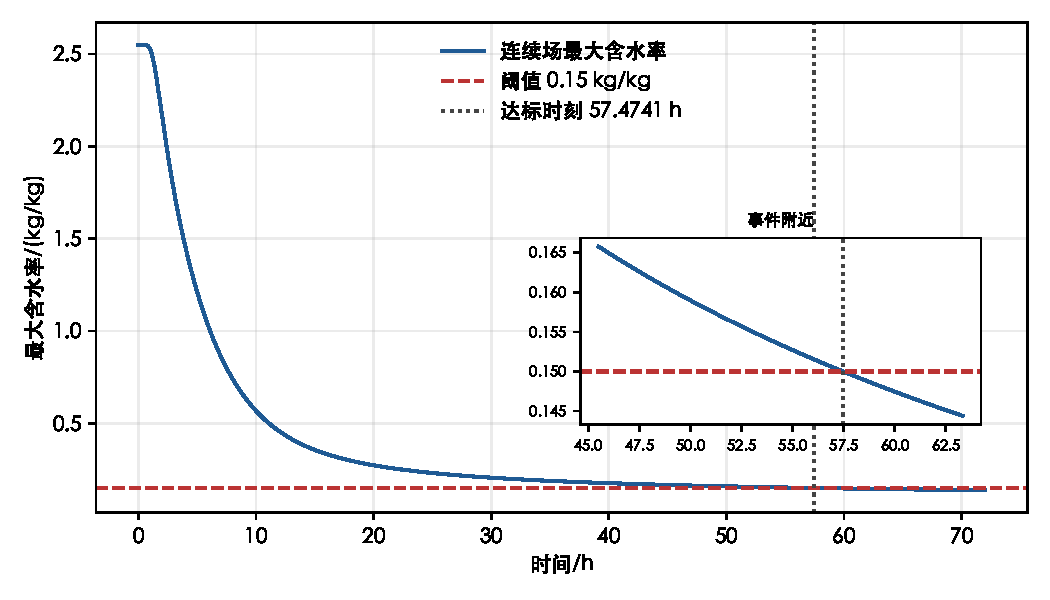
\includegraphics[width=0.82\textwidth]{../figures/q3/q3_threshold_event.pdf}
  \caption{问题三全域最大含水率与达标事件}
  \label{fig:q3event}
\end{figure}

\begin{table}[H]\centering\small\caption{问题三达标过程的典型位置含水率（kg/kg）}\label{tab:q3moisture}\begin{tabular}{rrrrrr}\toprule 时间/h&0 cm&0.5 cm&1 cm&1.5 cm&2 cm\\\midrule 6&1.0170&0.9881&0.9015&0.7550&0.5328\\12&0.4562&0.4432&0.4031&0.3297&0.1642\\18&0.2988&0.2916&0.2687&0.2253&0.0845\\24&0.2378&0.2327&0.2167&0.1855&0.0665\\30&0.2058&0.2018&0.1892&0.1641&0.0598\\36&0.1859&0.1825&0.1718&0.1504&0.0566\\42&0.1721&0.1691&0.1597&0.1407&0.0548\\48&0.1618&0.1592&0.1507&0.1334&0.0537\\54&0.1539&0.1514&0.1436&0.1277&0.0530\\57.4741&0.1500&0.1477&0.1402&0.1249&0.0526\\\bottomrule\end{tabular}\end{table}
表 5 的原始数据见 \texttt{results/q3/table5.csv}。网格 $N=256,512,1024$ 对应事件时刻为 57.47424678、57.47410135、57.47406473 h，收紧时间设置后变化为 $-0.198\,\mathrm s$。图~\ref{fig:q3event}展示阈值函数和事件根。
